% ─────────────────────────────────────────────────────────────────────────────
% CHAPTER 4: System Design
% ─────────────────────────────────────────────────────────────────────────────

This chapter translates the requirements specified in Chapter~3 into architectural, database, mathematical, and algorithmic designs. It details the high-level system tiers, data models, the autonomous agent workflow, the merchant quotation engine formulas, and real-time communication events.

\section{Architectural Evolution: 1-Tier, 2-Tier, and 3-Tier Models}

Before examining the detailed design of GroDealz, it is useful to review the architectural evolution from monolithic 1-tier and 2-tier client-server designs to the modern 3-tier architecture.

\subsection{1-Tier vs.\ 2-Tier Architectural Models}

Figure~\ref{fig:1tier_2tier} illustrates the fundamental differences between 1-tier and 2-tier architectures:

\begin{figure}[H]
\centering
\begin{subfigure}[b]{\linewidth}
  \centering
  \begin{minipage}[c]{0.50\linewidth}
    \centering
    \resizebox{0.92\linewidth}{!}{%
    \begin{tikzpicture}[node distance=0.45cm]
      \node[tierbox, fill=orange!10, draw=orange!70!black, minimum width=5.0cm, minimum height=0.6cm, align=center] (p1) {
        \textbf{Presentation Layer} (UI, Forms, Menus)
      };
      \node[tierbox, fill=green!10, draw=green!70!black, minimum width=5.0cm, minimum height=0.6cm, below=of p1, align=center] (a1) {
        \textbf{Application Logic} (Calculations / Validation)
      };
      \node[tierbox, fill=purple!10, draw=purple!70!black, minimum width=5.0cm, minimum height=0.6cm, below=of a1, align=center] (d1) {
        \textbf{Data Layer} (Local Files / SQLite DB)
      };
      
      \draw[arrowflow, shorten >= 2mm, shorten <= 2mm] (p1.south) -- (a1.north);
      \draw[arrowflow, shorten >= 2mm, shorten <= 2mm] (a1.south) -- (d1.north);

      \begin{scope}[on background layer]
        \node[tierframe, fill=gray!3, fit=(p1) (a1) (d1), label={[font=\scriptsize\bfseries, yshift=-2pt]above:Standalone Computer / Monolith}] {};
      \end{scope}
    \end{tikzpicture}%
    }
  \end{minipage}\hfill
  \begin{minipage}[c]{0.46\linewidth}
    \textbf{1-Tier Architecture:}\\[0.25em]
    \small All presentation interface, application logic, and database storage reside on a single standalone machine. It cannot support network collaboration, shared merchant inventory, or multi-buyer ordering.
  \end{minipage}
  \vspace{0.15cm}
  \caption{1-Tier Monolithic Model (Single Standalone Machine)}
  \label{fig:1tier}
\end{subfigure}

\vspace{0.5cm}

\begin{subfigure}[b]{\linewidth}
  \centering
  \begin{minipage}[c]{0.50\linewidth}
    \centering
    \resizebox{0.95\linewidth}{!}{%
    \begin{tikzpicture}[node distance=1.8cm]
      \node[tierbox, fill=blue!8, draw=blue!70!black, minimum width=2.4cm, minimum height=2.1cm, align=center] (client) {
        \textbf{Client Tier}\\[0.2em]
        \rule{2.0cm}{0.3pt}\\[0.25em]
        Presentation (GUI)\\[0.15em]
        +\\[0.15em]
        Business Logic\\[0.15em]
        DB Credentials
      };
      \node[tierbox, fill=purple!8, draw=purple!70!black, minimum width=2.4cm, minimum height=2.1cm, align=center, right=of client] (db) {
        \textbf{Database Tier}\\[0.2em]
        \rule{2.0cm}{0.3pt}\\[0.25em]
        Central Database\\[0.15em]
        Server (RDBMS)\\[0.15em]
        Shared Storage\\[0.15em]
        Tables \& Records
      };

      \draw[arrowflow, shorten >= 3mm, shorten <= 3mm] ([yshift=8pt]client.east) -- node[midway, above, font=\tiny, align=center] {SQL Query\\(ODBC/JDBC)} ([yshift=8pt]db.west);
      \draw[arrowflow, shorten >= 3mm, shorten <= 3mm] ([yshift=-8pt]db.west) -- node[midway, below, font=\tiny, align=center] {Result Dataset\\(Raw Records)} ([yshift=-8pt]client.east);
    \end{tikzpicture}%
    }
  \end{minipage}\hfill
  \begin{minipage}[c]{0.46\linewidth}
    \textbf{2-Tier Architecture:}\\[0.25em]
    \small Fat client machines connect directly over a local network to a central database server. It exposes database credentials inside the client binary and requires client upgrades whenever business logic changes.
  \end{minipage}
  \vspace{0.15cm}
  \caption{2-Tier Client-Server Model (Direct Database Connection)}
  \label{fig:2tier}
\end{subfigure}
\caption{Comparison of 1-Tier and 2-Tier Architectural Models with Functional Descriptions}
\label{fig:1tier_2tier}
\end{figure}

\begin{enumerate}
    \item \textbf{1-Tier Architecture (Monolithic):} In a 1-tier architecture, the presentation layer, application business logic, and database storage reside on the exact same physical computer (for example, a traditional desktop application using an embedded SQLite or Microsoft Access database). While this model requires zero network overhead, it is completely unsuitable for a multi-store grocery platform: multiple customers, store owners, and delivery riders cannot coordinate shared inventory, live orders, or real-time bids on a standalone machine.
    \item \textbf{2-Tier Architecture (Traditional Client-Server):} In a 2-tier architecture, the presentation interface and application business logic run together on a ``fat client'' machine, which communicates directly over a local network or VPN to a centralized database server using database connection protocols (such as ODBC or JDBC). While this enables shared data storage, it introduces critical vulnerabilities:
    \begin{itemize}
        \item \emph{Security Risk:} Embedding direct database credentials within the client application exposes the core database to tampering.
        \item \emph{Tight Coupling and Maintenance Burden:} Any modification to business logic, pricing rules, or quotation ranking algorithms requires updating the client software on every user's device.
        \item \emph{Poor Scalability for AI Tasks:} Complex computations---such as cross-store basket optimization and demand forecasting---would consume local client device memory and cannot easily leverage server-side parallelism.
    \end{itemize}
\end{enumerate}

\subsection{3-Tier Architecture of GroDealz}

To overcome these structural limitations, GroDealz implements a clean \textbf{3-Tier Architecture}, decoupling the Presentation Tier, the Application and AI Logic Tier, and the Data Persistence Tier. Figure~\ref{fig:3tier_arch} depicts the architectural tiers and the communication flows between them.

\begin{figure}[H]
\centering
\resizebox{\linewidth}{!}{%
\begin{tikzpicture}[node distance=4.0cm]
  % Tier 1
  \node[tierbox, fill=blue!6, draw=blue!70!black, minimum width=4.2cm, minimum height=5.2cm, align=center] (t1) {
    \textbf{\large Tier 1: Presentation}\\[0.2em]
    \textbf{\footnotesize (Frontend SPA)}\\[0.3em]
    \rule{3.8cm}{0.4pt}\\[0.4em]
    React 18 Single-Page App\\[0.25em]
    React Router v6 Navigation\\[0.25em]
    AuthContext \& CartContext\\[0.25em]
    Socket.IO Client Connection\\[0.25em]
    Axios HTTP Interceptor (JWT)\\[0.25em]
    Buyer RFQ \& Merchant Bids\\[0.25em]
    AI Copilot \& Store Tour UI\\[0.25em]
    Customer Support CRM
  };

  % Tier 2
  \node[tierbox, fill=green!6, draw=green!70!black, minimum width=4.8cm, minimum height=5.2cm, align=center, right=of t1] (t2) {
    \textbf{\large Tier 2: Application \& AI Logic}\\[0.2em]
    \textbf{\footnotesize (Node.js API + Python FastAPI)}\\[0.3em]
    \rule{4.4cm}{0.4pt}\\[0.4em]
    Express 4 REST Core Server\\[0.25em]
    JWT Authentication Middleware\\[0.25em]
    Module B Quotation Engine\\[0.25em]
    Python LangGraph Agent\\[0.25em]
    Hybrid Recommendation Engine\\[0.25em]
    Automated Demand Forecaster\\[0.25em]
    Socket.IO Room Dispatcher\\[0.25em]
    NLP Intent Classifier \& PII Mask
  };

  % Tier 3
  \node[tierbox, fill=purple!6, draw=purple!70!black, minimum width=4.2cm, minimum height=5.2cm, align=center, right=of t2] (t3) {
    \textbf{\large Tier 3: Data Layer}\\[0.2em]
    \textbf{\footnotesize (Persistence \& Schemas)}\\[0.3em]
    \rule{3.8cm}{0.4pt}\\[0.4em]
    MongoDB Atlas (Mongoose ODM)\\[0.25em]
    User \& Store Collections\\[0.25em]
    Product Catalog (Indexed)\\[0.25em]
    BuyerRequest Collection\\[0.25em]
    MerchantQuotation Bids\\[0.25em]
    Order Status History\\[0.25em]
    Support Tickets \& CRM Log\\[0.25em]
    Compound \& Text Indexes
  };

  % Arrows between Tier 1 and Tier 2 (shorten >= 6mm ensures arrowheads have generous daylight from box borders)
  \draw[arrowflow] ([yshift=18pt]t1.east) -- node[midway, above=2pt, font=\scriptsize, align=center] {HTTPS REST / JSON\\(JWT Bearer Token)} ([yshift=18pt]t2.west);
  \draw[arrowflow] ([yshift=-18pt]t2.west) -- node[midway, below=2pt, font=\scriptsize, align=center] {Socket.IO Push\\(Real-Time Sync)} ([yshift=-18pt]t1.east);

  % Arrows between Tier 2 and Tier 3 (shorten >= 6mm ensures arrowheads have generous daylight from box borders)
  \draw[arrowflow] ([yshift=18pt]t2.east) -- node[midway, above=2pt, font=\scriptsize, align=center] {Mongoose Queries\\(CRUD \& Filter)} ([yshift=18pt]t3.west);
  \draw[arrowflow] ([yshift=-18pt]t3.west) -- node[midway, below=2pt, font=\scriptsize, align=center] {BSON Result Sets\\\& Aggregations} ([yshift=-18pt]t2.east);

\end{tikzpicture}%
}
\caption{3-Tier High-Level Architecture of the GroDealz Platform. Tier~1 manages customer interactions in React~18, Tier~2 processes quotation algorithms and AI agents in Node.js/Python, and Tier~3 secures relational and document data in MongoDB Atlas.}
\label{fig:3tier_arch}
\end{figure}

The responsibilities of each tier are defined as follows:

\begin{enumerate}
    \item \textbf{Tier 1 --- Presentation Tier (Client):} Built as a lightweight, reactive Single-Page Application (SPA) using React 18. The presentation tier manages local state (such as the cart, user login status, active filters, and navigation paths) and renders the dark-mode responsive interface. It communicates with Tier~2 exclusively over secure HTTPS REST endpoints and persistent WebSocket channels, ensuring that no database credentials or internal business formulas are exposed to the client.
    \item \textbf{Tier 2 --- Application and AI Logic Tier (Server):} Implemented using Node.js with Express~4 and Python 3.10 with FastAPI/LangGraph. This tier acts as the centralized brain of the platform:
    \begin{itemize}
        \item \emph{Security \& Authentication:} Validates cryptographic JWT signatures on incoming requests and enforces role-based authorization (customer vs.\ store owner vs.\ admin).
        \item \emph{Quotation Engine (Module B):} Evaluates line-item mathematics, computes dynamic ranking scores across customer-selected criteria, manages counter-offers, and coordinates atomic order conversion.
        \item \emph{Autonomous Shopping Agent:} Executes LangGraph decision graphs to search cross-store catalogs, verify inventory, optimize multi-store baskets, and compile picking itineraries.
        \item \emph{Real-Time Event Dispatcher:} Manages Socket.IO connection rooms (\texttt{merchants\_rfq}, \texttt{rfq\_<id>}, \texttt{order\_<id>}) to broadcast instantaneous updates without client polling.
    \end{itemize}
    \item \textbf{Tier 3 --- Data Persistence Tier (Database):} Managed by MongoDB Atlas via the Mongoose Object Document Mapper (ODM). Tier~3 guarantees transactional persistence, document validation, and high-performance querying through compound indexes on frequently queried fields. Direct database access is strictly isolated to Tier~2 through private database URIs.
\end{enumerate}

\section{Database Design and Data Models}

The database schema connects seven primary collections, as illustrated in the Entity-Relationship Diagram in Figure~\ref{fig:er_diagram}.

\begin{figure}[H]
\centering
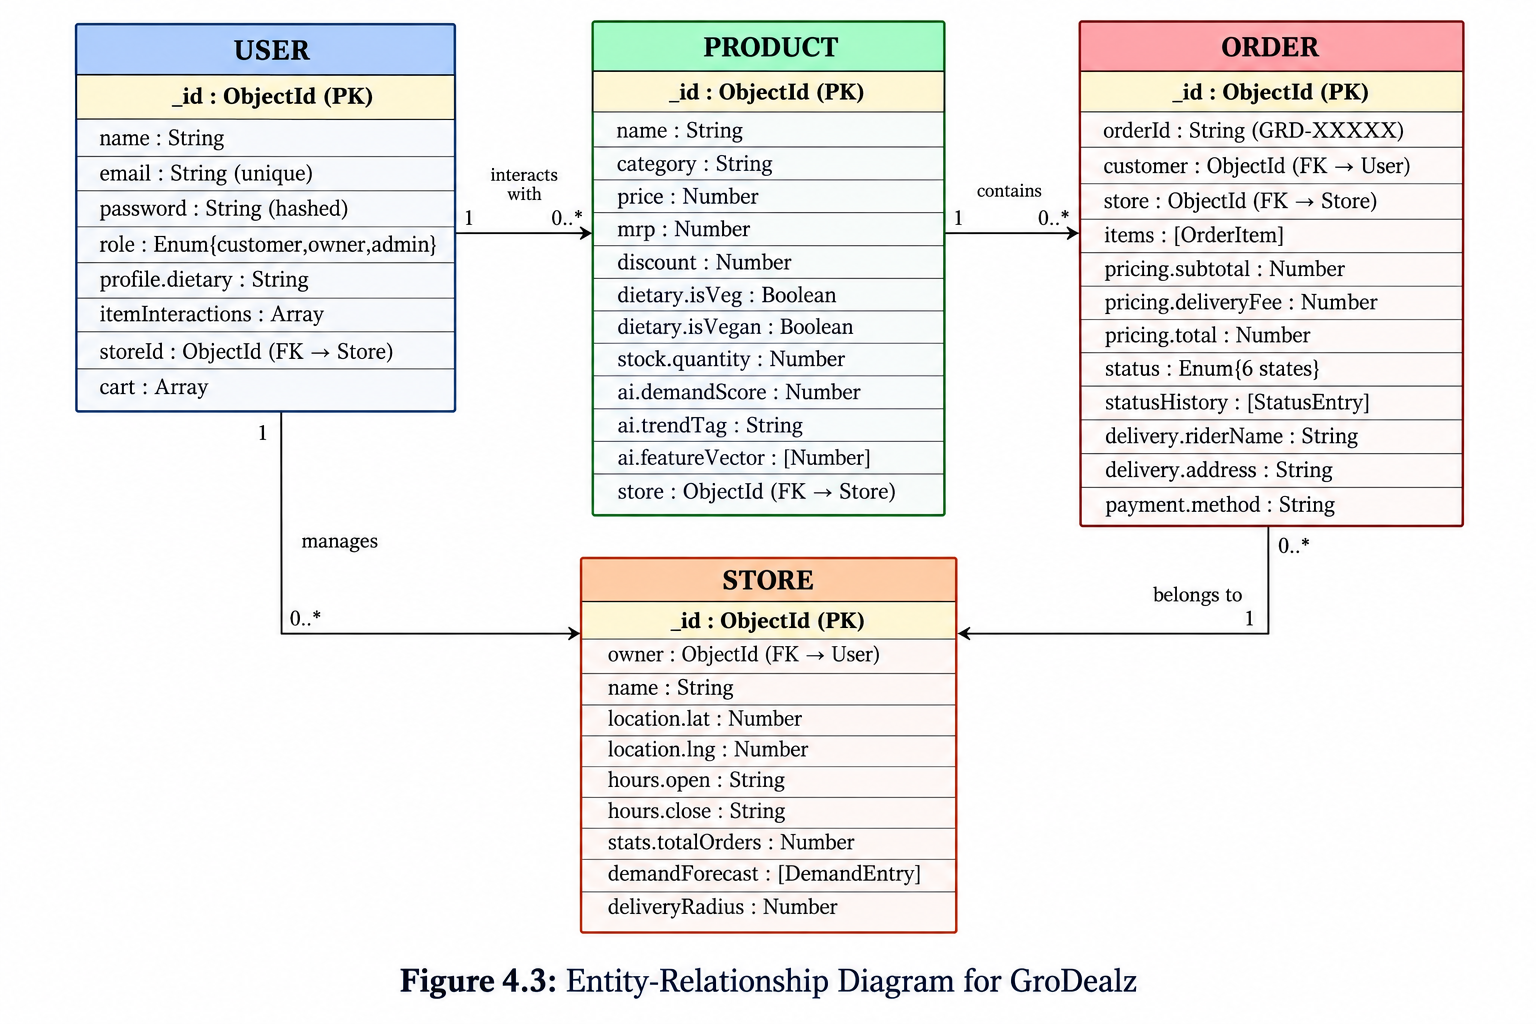
\includegraphics[width=0.92\textwidth,keepaspectratio]{figures/erd.png}
\caption{Entity-Relationship Diagram (ERD) of GroDealz Database. Illustrates relational dependencies across seven primary collections including User, Store, Product, Order, BuyerRequest, MerchantQuotation, and Customer Support.}
\label{fig:er_diagram}
\end{figure}

In addition to the standard User, Product, Store, and Order collections, GroDealz introduces two purpose-built schemas for the reverse marketplace:

\subsection{Buyer Request Schema}
Stores custom customer shopping requirements:
\begin{itemize}
    \item \textbf{Request Identifier (\textit{requestId}):} Unique identifier code (e.g., RFQ-20261031-4821).
    \item \textbf{Customer Reference (\textit{customer}):} Reference to the User ID of the buyer.
    \item \textbf{Requirement Title (\textit{title}):} Short requirement summary (e.g., ``25 kg Basmati Rice for Hostel'').
    \item \textbf{Raw Prompt (\textit{rawPrompt}):} Raw natural language prompt entered by the buyer.
    \item \textbf{Requested Items (\textit{items}):} Structured array of requested items with quantities, units, and brand preferences.
    \item \textbf{Target Budget (\textit{budget}):} Optional numerical target budget in Indian Rupees.
    \item \textbf{Budget Sharing Flag (\textit{shareBudgetWithMerchants}):} Boolean flag to share target budget with bidding merchants.
    \item \textbf{Delivery Deadline (\textit{deliveryDeadline}):} Required delivery completion timestamp.
    \item \textbf{Ranking Priority (\textit{rankingPriority}):} Chosen sorting criterion (price, delivery, rating, or balanced).
    \item \textbf{RFQ Status (\textit{status}):} Current state (\textit{open}, \textit{quotes\_received}, \textit{negotiating}, \textit{accepted}, \textit{expired}).
    \item \textbf{Converted Order Reference (\textit{convertedOrderId}):} Reference to the created order when quotation is accepted.
\end{itemize}

\subsection{Merchant Quotation Schema}
Stores itemized quotations submitted by competing store owners:
\begin{itemize}
    \item \textbf{Quotation Identifier (\textit{quotationId}):} Unique identifier code (e.g., QUO-20261031-1049).
    \item \textbf{Parent Request Reference (\textit{request}):} Reference to the parent Buyer Request.
    \item \textbf{Store and Merchant References (\textit{store}, \textit{merchant}):} References to the merchant store and user account.
    \item \textbf{Quoted Line Items (\textit{lineItems}):} Array of quoted line items with unit price, stock status, and line totals.
    \item \textbf{Financial Totals (\textit{itemsSubtotal}, \textit{deliveryCharge}, \textit{tax}, \textit{grandTotal}):} Transparent cost breakdown.
    \item \textbf{Stock Confirmation Flag (\textit{stockConfirmed}):} Boolean indicating immediate inventory reservation.
    \item \textbf{Delivery Schedule and Validity (\textit{proposedDeliveryDate}, \textit{expiresAt}):} Proposed delivery date and offer expiry.
    \item \textbf{Buyer Counter-Offer Subdocument (\textit{counterOffer}):} Subdocument storing buyer counter-offer and negotiation note.
    \item \textbf{Revision History (\textit{revisionHistory}):} Historical audit log of updated quote versions.
\end{itemize}

Figure~\ref{fig:uml} shows the UML Class Diagram highlighting the relationship between these domain models and service engines.

\begin{figure}[H]
\centering
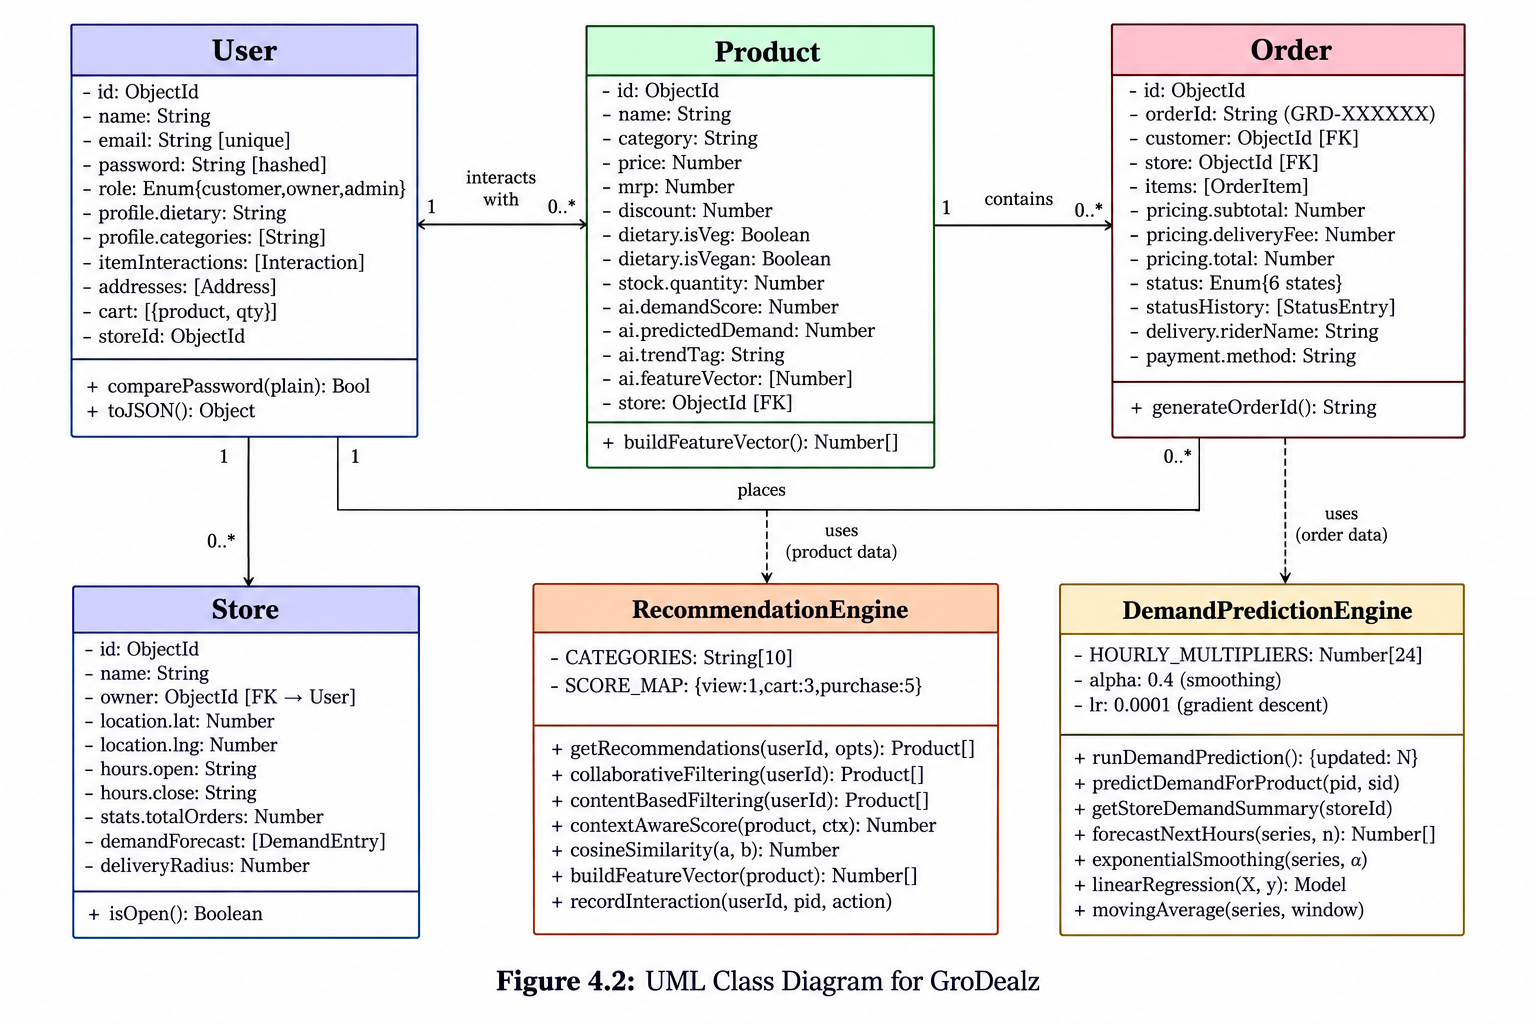
\includegraphics[width=0.92\textwidth,keepaspectratio]{figures/uml.png}
\caption{UML Class Diagram of System Architecture. Details domain model schemas, controller interfaces, algorithmic quotation engines, and real-time Socket.IO notification rooms.}
\label{fig:uml}
\end{figure}

\section{Autonomous AI Shopping Agent Workflow}

The Autonomous AI Grocery Shopping Agent (accessible on \texttt{/ai-planner}) operates as a state-machine graph implemented via LangGraph. When a user submits an informal shopping goal (such as \emph{``Party snacks and beverages for 5 people under ₹600''}), execution proceeds through five sequential nodes:

\begin{enumerate}
    \item \textbf{Parameter Extraction Node:} Employs structured natural language parsing to extract the target count of individuals ($N=5$), planning duration ($D=3\text{ days}$), maximum target budget ($B=₹600$), dietary constraints, and item categories.
    \item \textbf{Cross-Store Discovery Node:} Queries participating local merchant databases (e.g., FreshMart Central, QuickBazaar, Paona Supermarket) to assemble candidate products matching each needed category.
    \item \textbf{Fresh Stock Verification Node:} Verifies current shelf quantities and freshness indicators, filtering out items that are out of stock.
    \item \textbf{Basket Optimization Node:} Solves the single-store versus multi-store tradeoff. Buying all items from one convenient store incurs a single delivery fee ($F_{\text{single}}$), whereas splitting items across multiple stores allows selecting the minimum product price $P_{s, i}$ from store $s$ at the cost of separate store delivery charges $F_s$:
    \begin{align}
        &C_{\text{single}} = \sum_{i \in I} P_{\text{single}, i} + F_{\text{single}} \\
        &C_{\text{multi}} = \sum_{s \in S_{\text{visited}}} \left( \sum_{i \in I_s} P_{s, i} + F_s \right) \\
        &\Delta_{\text{savings}} = C_{\text{single}} - C_{\text{multi}}
    \end{align}
    If $\Delta_{\text{savings}} > 0$, the multi-store split is recommended to the customer as the best-value deal.
    \item \textbf{Store Journey Audit Node:} Generates an audit trail detailing the exact items to pick at each shop and visualizes the itinerary in the user interface.
\end{enumerate}

\section{Module B Quotation Engine Design}

The Merchant Quotation Engine governs the pricing, ranking, and negotiation lifecycle of custom shopping requirements.

\subsection{Itemized Pricing Calculations}
Merchants cannot simply quote an arbitrary lump sum; they must submit unit prices for every individual line item requested. This ensures transparency for the customer:
\begin{align}
    &\text{lineTotal}_i = \text{quantity}_i \times \text{unitPrice}_i \\
    &\text{itemsSubtotal} = \sum_{i=1}^n \text{lineTotal}_i \\
    &\text{grandTotal} = \text{itemsSubtotal} + \text{deliveryCharge} + \text{tax}
\end{align}

\subsection{Multi-Criteria Dynamic Ranking Formulations}
Unlike standard platforms that sort solely by price, GroDealz allows customers to rank bids based on their immediate priority:

\begin{enumerate}
    \item \textbf{Lowest Price Mode (\textit{lowest\_price}):} Evaluates grand total cost. The lowest grand total receives the highest ranking score:
    \begin{equation}
        \text{Score}_{\text{price}} = 1{,}000{,}000 - \text{grandTotal}
    \end{equation}
    The merchant with the minimum total is awarded the badge \emph{``Lowest Total Price.''}
    
    \item \textbf{Fastest Delivery Mode (\textit{fastest\_delivery}):} Evaluates the proposed delivery timestamp ($t_{\text{delivery}}$). Bids proposing earlier delivery receive higher scores:
    \begin{equation}
        \text{Score}_{\text{delivery}} = T_{\text{future}} - t_{\text{delivery}}
    \end{equation}
    The earliest delivery bid receives the badge \emph{``Fastest Delivery.''}
    
    \item \textbf{Top Rated Store Mode (\textit{highest\_rated}):} Prioritizes merchant reliability based on customer reviews and ratings:
    \begin{equation}
        \text{Score}_{\text{rating}} = (\text{Rating} \times 1{,}000) + \min(\text{ReviewCount}, 100)
    \end{equation}
    The highest-rated vendor is highlighted with the badge \emph{``Top Rated Store.''}
    
    \item \textbf{Balanced Composite Mode (\textit{balanced}):} Combines price, delivery speed, and store reputation into a normalized 100-point composite score:
    \begin{equation}
        \text{Score}_{\text{balanced}} = S_{\text{price}} (50\text{ pts}) + S_{\text{speed}} (30\text{ pts}) + S_{\text{reputation}} (20\text{ pts})
    \end{equation}
    where:
    \begin{align}
        &S_{\text{price}} = 50 \times \left( 1 - \frac{\text{grandTotal} - \text{minPrice}}{\text{maxPrice} - \text{minPrice}} \right) \\
        &S_{\text{speed}} = 30 \times \left( 1 - \frac{t_{\text{delivery}} - t_{\text{earliest}}}{t_{\text{latest}} - t_{\text{earliest}}} \right) \\
        &S_{\text{reputation}} = \left( \frac{\text{Rating}}{5.0} \right) \times 20
    \end{align}
    If the quoted total is within the customer's target budget, an additional 5-point bonus is applied.
\end{enumerate}

\section{Real-Time WebSocket Event Architecture}

To provide instantaneous notifications without inefficient browser polling, GroDealz utilizes Socket.IO rooms:
\begin{itemize}
    \item \textbf{Request Notification Room (\textit{join\_rfq}):} Customer joins a private room for their request. When a merchant submits or revises a quote, the server emits a \textit{quote\_update} event.
    \item \textbf{Merchant RFQ Broadcast Room (\textit{join\_merchants\_rfq}):} Merchants join a collective broadcast room. When a customer posts a new requirement, the server emits a \textit{new\_rfq\_available} notification.
    \item \textbf{Order Status Tracking Room (\textit{track\_order}):} Customers track real-time order status transitions (\emph{placed $\to$ confirmed $\to$ delivered}).
\end{itemize}
